\problemname{Mosaic Mansion}

A mosaic is a picture made from square tiles arranged in a grid, at least for
today's purposes.

We would like to make a mosaic with exactly the same number of tiles of each
colour. We will do this by taking an existing design and removing some of the
rows from it.

\begin{figure}[h!]
  \centering
  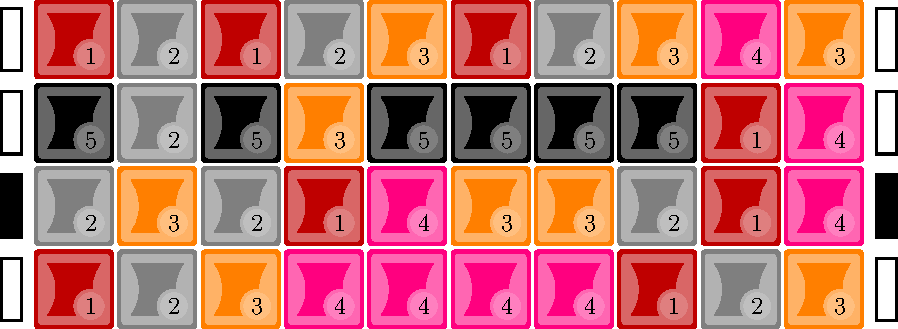
\includegraphics[width=1.0\textwidth]{sample}
  \caption{Illustration of a solution to Sample Input 1. The three rows
  annotated with white can be kept, giving $6$ of each colour of tile.}
  \label{fig:mosaic}
\end{figure}

What is the greatest number of rows we can keep?

\section*{Input}

\begin{itemize}
  \item The first line of input contains
        the number of rows, $n$ ($1 \le n \le 40$),
        the number of columns, $m$ ($1 \le m \le 10^5$), and
        the number of colours, $c$ ($1 \le c \le 10^5$) in the mosaic
        respectively.
  \item Each of the next $n$ lines contains $m$ colours of cells
        $p_1 \ldots p_m$ ($1 \le p \le c$).
\end{itemize}

\section*{Output}

Output the greatest number of rows that can be kept while keeping equal
representation for each colour in the input, or $0$ if no rows can be kept.
